\documentclass[11pt]{article}
\usepackage{amssymb}
\usepackage{algpseudocode}
\usepackage{algorithm}
\usepackage{setspace}
\usepackage{graphicx}
\graphicspath{ {./images/} }
\usepackage{hyperref}
\usepackage{siunitx}
\usepackage{amsmath}
\usepackage{caption}
\usepackage{subcaption}

\hypersetup{
    colorlinks=true,
    linkcolor=blue,
    filecolor=magenta,      
    urlcolor=cyan,
}

\title{MSc Project - Binding Affinity Prediction of Protein-Ligand Complex}
\author{
        Abdus Salam Khazi\\
        \href{mailto:abdus.khazi@students.uni-freiburg.de}
                {abdus.khazi@students.uni-freiburg.de}\\ \\
        \href{https://github.com/abduskhazi/MSc-Project}
                {Github Repository} \cite{github_repository} \\ \\
        Supervisors:
        \begin{tabular}{ll}
			Simon Bray \&
			Alireza Khanteymoori
		\end{tabular}
       }
	
\begin{document}

\maketitle
\date{}
\tableofcontents
\newpage

\section{Abstract}
\newpage

\section{Introduction}

\subsection{Biological Background}
Proteins are the workhorses of our body.  They are necessary for many important functions in the body.  Ligands are molecules that bind to proteins to form protein-ligand complexes.  They can be molecules that the protein transports (e.g., a Haemoglobin transporter) or act as stimulating agents.  In addition to this, they can also start/stop the protein from doing its function.  The correct functioning of these protein-ligand complexes is essential for any living organism.

The study of protein-ligand complexes is an intrinsic part of the drug discovery field.  It is because drugs are small molecules that act as ligands.  As the drug molecules (ligands) bind to the target proteins, they can artificially influence the protein behavior.  This binding between protein and ligand causes a therapeutic effect.

\begin{figure}[htb]
  \centering
    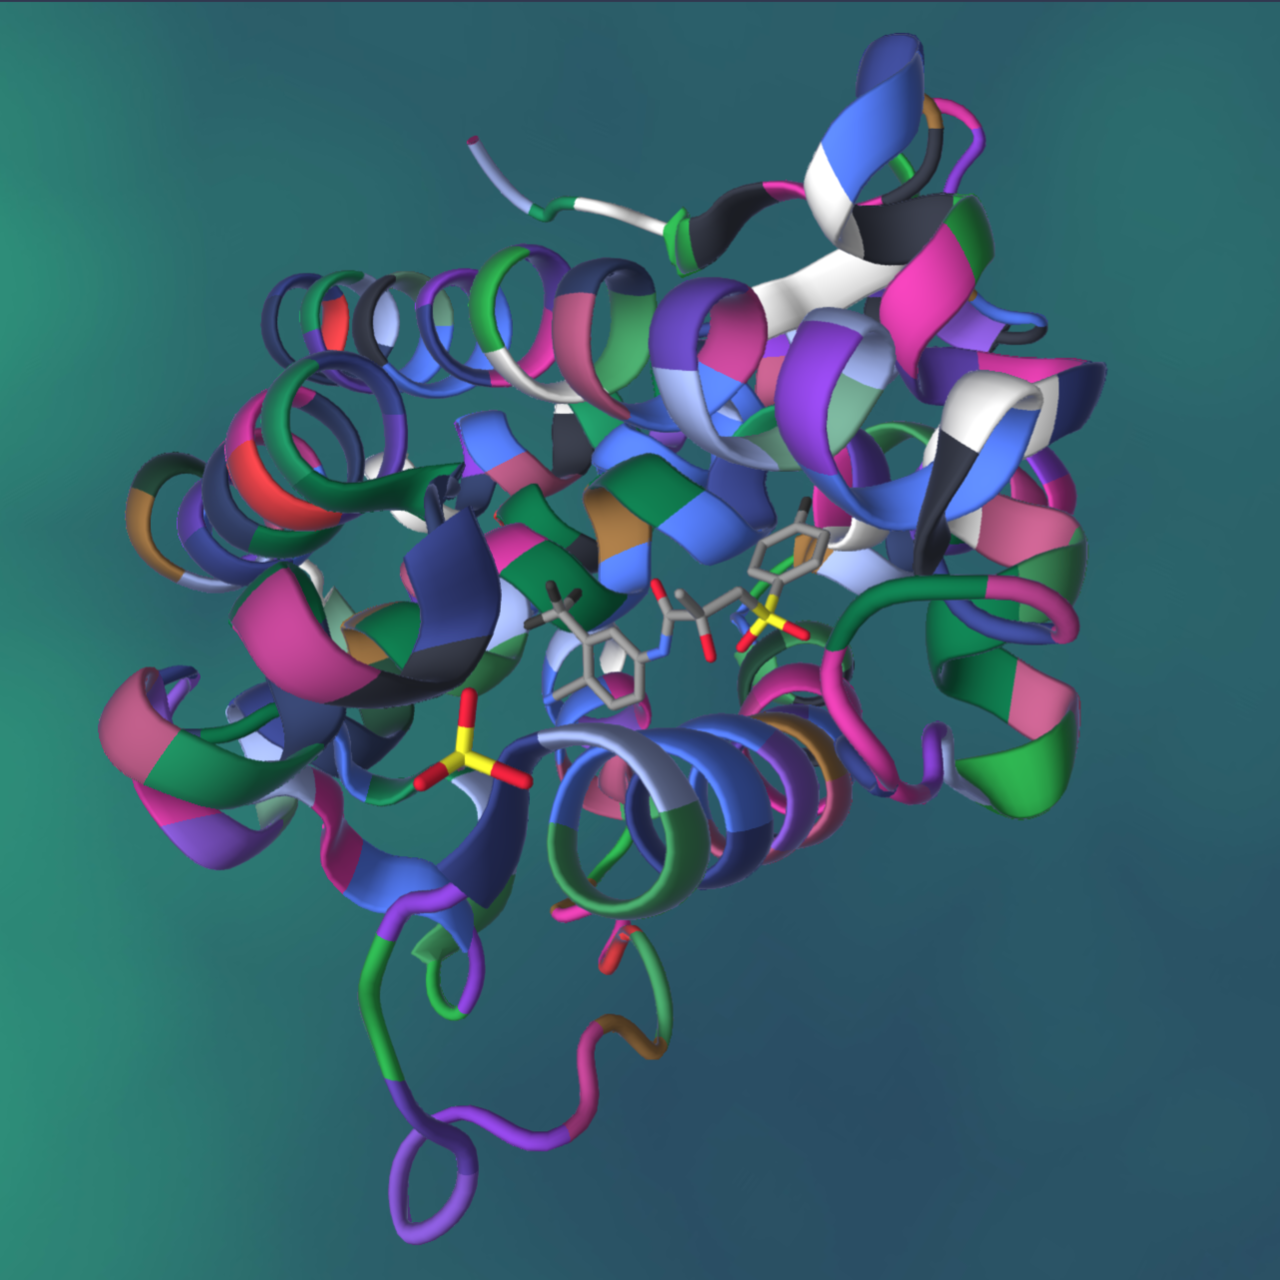
\includegraphics[scale=0.15]{images/pl_complex}
    \caption{Haemoglobin transporter protein.  \cite{PL_complex_introduction}}
    \label{fig:HaemoglobinTransporterImage}
\end{figure}


When we find a target drug candidate, we have to answer questions like - How easily does the drug bind to the target protein? Does it bind to any other protein - If so, is it desirable? Does it have any unforeseen effect on the protein function? etc...  To answer these questions biologists and pharmacists conduct wet-lab experiments that are expensive.

One way to reduce the cost of these experiments is to make a data-driven selection of the drugs.  Using experimental data collected over many years, one can build models to predict the behavior of the proposed drug computationally.  These 'In-Silico' computational methods can aid in the elimination of undesirable drugs as well as guide the drug selection process.

Our project aims to answer one of the above questions - How well does a given drug bind to the target protein? We determine this computationally by building a machine learning model that trains on the previous data.  We hope that this model will help reduce the costs of drug discovery. 

\subsection{Understanding Binding Affinity}
The binding affinity between a protein and a ligand is quantified by the $K_d$, $K_i$ and $IC_{50}$ measures in the PDBBind Data bank.
Here $K_d$ refers to disassociation constant, $K_i$ refers to the inhibition constant, and $IC_{50}$ refers to 
inhibitory concentration 50\%.
The reason for having different measurements is because it is not possible to use the same measurement techniques
for all biological complexes/processes.

To understand $K_d$, consider a protein and a ligand binding and unbinding continuously in a kinetic system.
In this system, let $[P]$, $[L]$, and $[PL]$ represent the concentrations of the Protein, the Ligand, and the Protein-Ligand complex respectively.
This is represented by the following equation:
$$[P] + [L] \rightleftharpoons [PL]$$
We can quantify the binding affinity $K_d$ by using the concentrations in the above system at equilibrium.
$$K_d = \frac{[P][L]}{[PL]} = \frac{k_{-1}}{k_1}$$
where $k_{-1}$ is the disassociation rate constant and $k_1$ is the association rate constant.
Similarly, $K_i$ and $IC_{50}$ are defined using concentration albeit non-trivially. 
\cite{binding_affinity_description}

\subsection{PDBBind Dataset}
Over the last few decades, researchers have been successful in building a single data archive for proteins.  This archive, called \textbf{Protein Data Bank} \cite{pdb_homepage} , holds 3-D structural data of the proteins determined by experiments like X-ray crystallographic, Nuclear magnetic resonance (NMR), and cryoelectron microscopy (cryoEM).  A subset of this data also contains information about how well a given protein and ligand bind together.  It is called binding affinity between a protein and ligands.  (It also contains data about protein-protein complexes that our project does not deal with)
\cite{pdbank_history}

As we study the protein-ligand binding affinity here, we would like to filter out this data from the \textbf{Protein Data Bank}  It is what is done by the maintainers of the \textbf{PDBBind Data Bank}.
\cite{pdbbind_introduction}
Using the curated protein-ligand affinity data present in the PDBBind Data bank, we build a machine learning model that learns to predict the affinity. 

\section{Problem Formulation}
\subsection{Problem Overview}
\label{ProblemOverviewlabel}
The problem that we are solving is - \textit{Given $K_d$/$K_i$/$IC_{50}$ for various complexes in the PDBBind Data bank,
can we predict this affinity measure for new protein-ligand complexes?}
Figure~\ref{fig:plproblemclassification} shows how the Protein-Ligand problem can be classified.

\begin{figure}[htb]
  \centering
    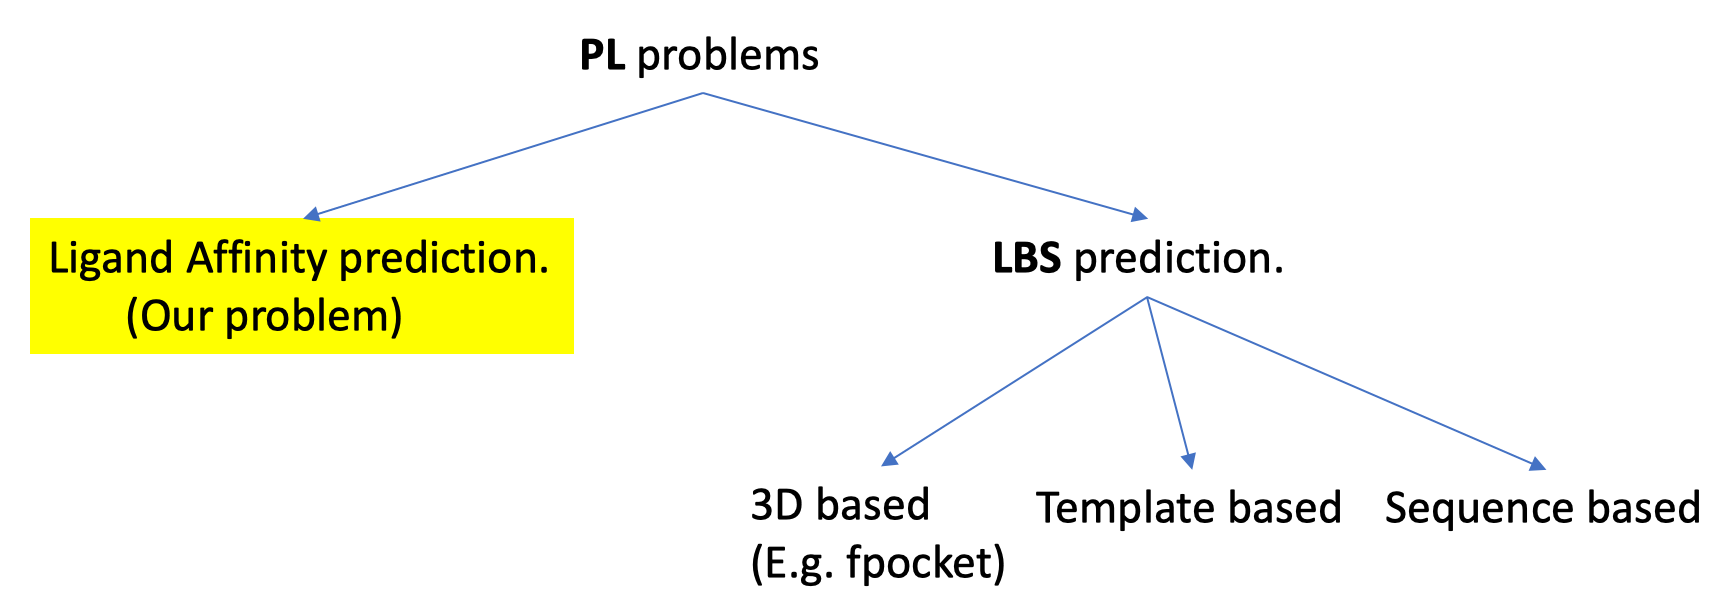
\includegraphics[scale=0.35]{images/pl_problem_classification}
    \caption{Protein-Ligand problem classifcation.}
    \label{fig:plproblemclassification}
\end{figure}

The binding of proteins and ligands is heavily influenced by their respective 3D structures.
Figure~\ref{fig:lockandkey} illustrates a hypothesis called \textit{Lock and Key}.
It is very crucial that the shape of the protein's binding location and the shape of the ligand be complementary for the binding.

\begin{figure}[htb]
  \centering
    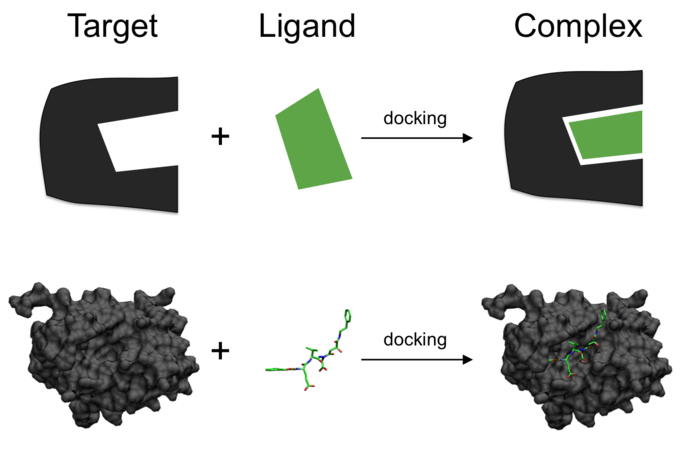
\includegraphics[scale=0.7]{images/lock_and_key}
    \caption{Lock and Key hypothesis in molecular docking.  \cite{lockandkeyformatpng}}
    \label{fig:lockandkey}
\end{figure}

The other parts of the protein are not involved in the binding process directly.
Hence,  we only get the features of the binding location.
Any potential binding location in the 3D structure of a protein is called a pocket.
We use a 3D based LBS prediction package called \textit{fpocket} to find the potential pockets.
A submodule in the package called \textit{dpocket} is used to extract the binding pocket's features.

To give a plug-and-play input to our model, we keep the features of proteins and ligands distinct till the training phase.
That is,  we do not use the combined features in any pre-processing of the ML pipeline e.g.  feature reduction.
This helps our model to provide the binding affinity between any protein and any ligand.



\subsection{Overview of file formats}
The \textbf{PDBBind Data bank} extracts information about the PL complexes from the \textbf{Protein Data bank} and creates the following files for every complex
\begin{itemize}
\item \textbf{PDB Format} - For the Protein.
\item  \textbf{Mol2} - For the ligand.
\item \textbf{SDF} - For the ligand.
\end{itemize}

All of the above formats contain the 3D information that is essential in the prediction of the binding affinity.
All the above mentioned formats use the \textbf{XYZ format} internally to represent the 3D structure of their molecules.

\subsubsection{XYZ format}
\label{xyz_format}
XYZ format is a chemical file format that represents the geometry of a molecule.
It specifies the number of atoms and their Cartesian X, Y, Z coordinates hence the name XYZ format.
The following text illustrates the XYZ format.
Section \ref{XYZFileexampleref} gives an example.
\cite{XYZ_format}
\begin{verbatim}
<number of atoms>
comment line
<element> <X> <Y> <Z>
...
\end{verbatim}

The unit of distance used is Angstrom (\si{\angstrom}).  \SI{1}{\angstrom} $ = 10^{-10}$ m.
\cite{XYZ_format}

\subsubsection{PDB format}
PDB format is a human-readable file format used to represent the protein molecules (macromolecules).
Within the PDB format,  the coordinates of atoms are represented like the XYZ format [see \ref{xyz_format}].
Because of the 3D information in this format,  molecular visualization of proteins is possible with specialized software. 
It also contains information about atomic connectivity and the protein's primary,  secondary,  tertiary,  and quaternary structures.
\cite{pdb_file_format}
\cite{understanding_pdb_format}
Please see \cite{examplePDBFile} for an example pdb file.


\subsubsection{Structure Data File (SDF) Format}
SDF format file is a Chemical Table file (CT File) that contains structure of the molecule in the X,Y,Z format.
It contains information like atomic bonds,  connectivity information,  molecular weight,  and molecular formula. \cite{SDFformat}
Section \ref{SDFFileexampleref} illustrates the SDF file format.

\subsubsection{Mol2 format}
Similar to SDF format,  Mol2 also represents the 3D structure of a molecule in the X,Y,Z format.
It contains the atomic bond and connectivity information but does not contain the other data like molecular weight and formula.
We use the ligands given in this format because more ligands in mol2 format could be processed with the RDKit feature extractor.
Section \ref{MOL2Fileexampleref} illustrates the Mol2 file format.

\subsubsection{SMILES format}
SMILES is an acronym for Simplified Molecular-Input Line-Entry System.
It represents a molecule using an ASCII string.
Using the 3D data in SDF and Mol2 formats,  we can create an atomic graph representation.
Using this graph the SMILES string for the molecule can be generated.
The SMILES format itself is not very helpful for us as we lose the 3D structural information after converting to it.
\cite{smilesformat}

\subsection{Extraction of features}
As the file formats are different for proteins and ligands,  we use different tools to extract their features.
\subsubsection{Ligand Features using RDKit}
RDKit is an open-source cheminformatics software \cite{rdkitofficalpage}.
The core data structures and algorithms of RDKit are written in C++ and the
python wrappers are generated using Boost.Python.
Using the module, \textit{RDKit.Chem.Descriptors} we extract $402$ features for each ligand \cite{rdkitbioinformaticsfreiburg}.
Each descriptor value is taken as a real number,  hence the input space of ligand features is $\mathbf{R}^{402}$ before any feature elimination.

\subsubsection{Protein Features using fpocket/dpocket descriptors}
\textit{Fpocket} stands for "Find pocket" whereas \textit{Dpocket} stands for "Describe pocket".
\textit{Fpocket} uses 3D Voronoi tessalation and the concepts of "Alpha Spheres" to find out pockets in the protein structure \cite{fpocketmanual} \cite{voronoitesselationshortvideo}.
Given a protein PDB file, we can extract the descriptors of all pockets in the protein.
For every pocket, we get 55 descriptors in total which are taken as real values,  $\mathbf{R}$.
Hence the input space for protein features is $\mathbf{R}^{55}$.


To get the descriptors of the ligand-binding pockets,  we use \textit{Dpocket}.
\textit{Dpocket} is provided with the protein PDB file and the ligand ID of the PL complex as input.
It generates 3 files as output files,  namely,  dpout\_fpocketp.txt, dpout\_fpocketnp.txt,  and  dpout\_explicitp.txt.
\begin{itemize}
\item \textbf{dpout\_fpocketp.txt}.
This file contains the descriptors (a.k.a features) of all pockets that are considered to be binding pockets based on a binding criterion.
The ligand can bind at different locations (pockets) in the protein 3D structure.
Hence,  there may be features of more than 1 pocket in this file.
\item \textbf{dpout\_fpocketnp.txt}.  This file contains the descriptors of all pockets that are non-binding according to the criteria.
\item \textbf{dpout\_explicitp.txt}.  An explicit pocket is defined as a pocket consisting of all vertices/atoms situated at a specific distance from the ligand in the PL complex.
This distance is 4 \r{A} by default.
This file contains the descriptors of all explicit pockets in the PL complex. 
\end{itemize}

In our project, we do not use dpout\_fpocketnp.txt as they contain non-binding pockets.
In the other 2 files,  we prefer using pocket descriptors given by dpout\_fpocketp.txt as explicitly defined pockets are heavily biased towards the ligand.

\section{Feature selection}
\subsection{Requirement of feature selection}
Both the protein and the ligand are equally responsible for the affinity of the PL complex.
Hence we concatenate their descriptors to get a high dimensional $\mathbf{R}^{457}$ input for our model.
There are a couple of issues with using all of the descriptors.
\begin{itemize}
\item The amount of data is not very large. 
For example,  we could only get $\approx$ 35000 data points after concatenating the ligand features with the \textit{fpocketp} pocket descriptors.
\item The number of ligand descriptors $>>$ protein descriptors.
This creates a data imbalance and may lead the model to select only ligand features for their prediction.
\end{itemize}
Hence we need some methods to reduce the input dimensions.

\subsection{Feature Family analysis}
\label{CorrelationAnalysis}
All the features extracted from the pdb and the ligand files can be classified into various families.
Some of the important ones are - AUTOCORR2d\_, Chi, EState\_VSA,  PEOE\_VSA,  SMR\_VSA,  SlogP\_VSA,  VSA\_EState and fr\_.
Figure~\ref{fig:correlationheatmap} shows correlation matrix of 2 of the most interesting families AUTOCORR2d\_ and Chi.
As we can see from the heatmap there is heavy correlation within the families.
Hence we also require a strategy to deal with this.
The correlation heat maps for the other families are illustrated in Section \ref{CorrHeatMapsAppendix}.

\begin{figure}[htb]
    \begin{subfigure}[b]{0.45\textwidth}
         \centering
         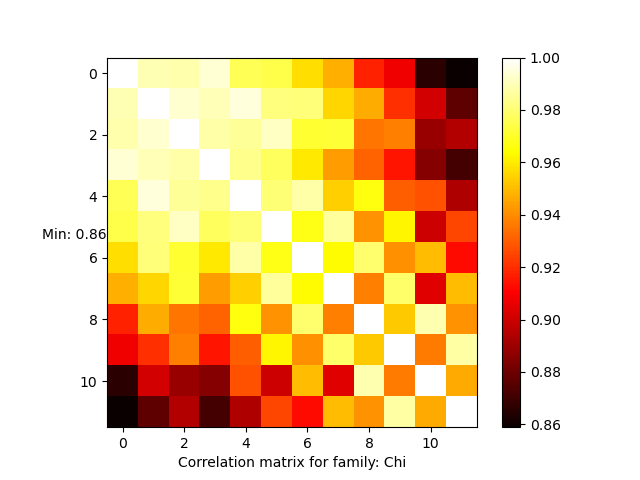
\includegraphics[scale=0.45]{images/correlationChi}
        \label{fig:correlationChi}
     \end{subfigure}
     \hfill
    \begin{subfigure}[b]{0.45\textwidth}
         \centering
         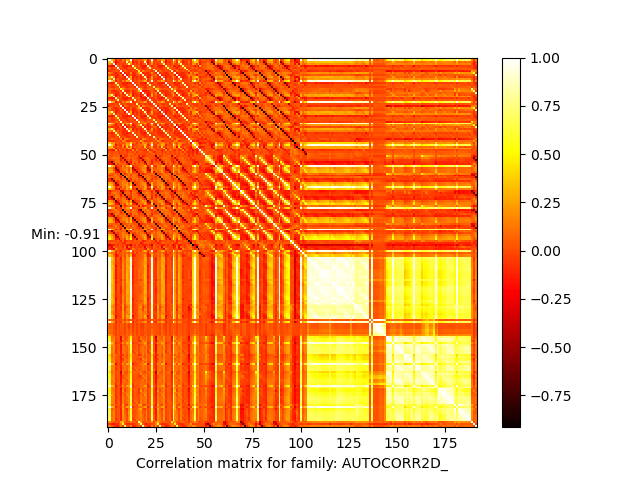
\includegraphics[scale=0.45]{images/correlationAUTOCORR2D}
        \label{fig:correlationfr}
     \end{subfigure}
     \caption{Correlation Heat Map}
     \label{fig:correlationheatmap}
\end{figure}

\subsection{Feature Selection Strategies}

%The data if it is complementary is better for solving the problem.
%The accuracy measure of the protein LBS prediction is the same as the dichotomous problems in math.

We try to select features of the protein and the ligand separately.
This helps us make our model plug-and-play as discussed in section \ref{ProblemOverviewlabel}.
The best combination,  i.e Global Optima,  cannot be obtained practically by brute force algorithms.
This is because we would have to try $\binom{402}{k_1} * \binom{55}{k_1}$ ($k_1, k_2 \in \mathbf{I}^+$) possibilities which is impractical.
In the next subsections we discuss a few feature selection strategies that were considered in our project.

\subsubsection{Selection by output correlation}
The \textit{pearson} and \textit{spearman} correlations of each feature were calculated against the output variable.
We assumed that the features were either linearly related to the output (in the case of Pearson correlation) or had a monotonic relationship (in the case of Spearman correlation).
The features with the highest correlation were selected as inputs to the model.

\subsubsection{Using genetic algorithms \cite{genetic_algorithm}}
Since the feature space is a non-continuous problem of combinatorial complexity,
we also studied genetic feature selection algorithms.
We represent each feature by a binary number, 1 for the inclusion of the feature and 0 for the exclusion.
Let $\mathbb{B}$ be a binary number $\{0,  1\}$.
Each feature selection $p \in \mathbb{B}^{456}$ (401 for ligands + 55 for proteins) is called a chromosome.
A "population" of $n$ chromosomes is maintained.
For each generation,  the best pairs of chromosomes are selected as parents.
The next generation is created by crossover and mutation of the chromosomes.
Algorithm~\ref{alg:GeneticAlgo} below gives complete pseudocode for this.

The scoring function used to select the best chromosome can vary according to the type of the model being fit. [See Section~\ref{MachineLearningModelslabel}]

\begin{algorithm}
\caption{Selection of features in our model using genetic algorithm \cite{genetic_algorithm}}
\label{alg:GeneticAlgo}
\begin{algorithmic}[1]
\Procedure{GENETIC\_ALGORITHM\_BASED\_SELECTOR}{}
\State scoringfunction $\gets$ Get model specific scoring function
\State $ population = \{C_1, C_2, C_3... C_n\}$ $\in$ $\mathbb{B}^{456}$ (initial chromosomes).
\State best $\gets C_1$  \textit{// Arbitrarily initialized}
\State $i \gets 0$
\State $gen \gets$ number of generations to run.
      \For{\texttt{$i < gen$ with step 1}}
          \State $\{S_1, S_2, S_3... S_n\} \gets$ scoringfunction($population$) $\forall S_i \in \mathbf{R}$.
          \State \textit{// Do a tournament selection for the best chromosomes}
          \State $genetically\_better\_population \gets$ empty list
          \For{\texttt{$j < len(population)$}}
              \State Set $\gets$ random\_k\_selections($population$)
              \State $c \gets best($Set$)$ \textit{// Based on scoringfunction.}
              \State $genetically\_better\_population.add(c)$
          \EndFor
          \State $children \gets$ empty list
          \For{\texttt{$j < len(population)$ with step 2}}
              \State $P_1, P_2$ $\gets$ $population[j], population[j+1]$
              \State $c_1, c_2 \gets crossover(P_1, P_2)$
              \State $c_1 \gets mutation(c_1)$
              \State $c_2 \gets mutation(c_2)$
              \State $children.add(c_1, c_2)$
          \EndFor
          \State $population \gets children$
      \EndFor
\State return best($population$)
\EndProcedure
\end{algorithmic}
\end{algorithm}

\subsubsection{Manual Feature selection}
A selected list of features were given to us by Simon Bray. 
We investigated manually selected 121 ligand descriptors. 
We continued to use all of the protein descriptors as they were only a few in number as compared to the ligand descriptors.

\section{Testing}
\subsection{Reproducibility}
Reproducible ML models are very crucial for verifying any project or research results. Due to the stochastic nature of many ML training processes, reproducing the exact model (and consequently the exact output) is a challenge. Two methods can be employed to produce verifiable results:
\begin{itemize}
\item Training many models and reporting the average results.
\item Controlling the randomness of the trained models. It is done by setting the seed of the pseudo-random algorithms.
\end{itemize}

We use the second approach in our project. Every script, when executed, reports an execution ID. This is the random seed used during the execution. If we want to reproduce the exact results, we give this execution ID to the script as the first argument.

\subsection{Model Quality Analysis}
We are trying to predict the following function
$$ \textrm{Binding affinity prediction} : \mathbf{R}^n \mapsto \mathbf{R} \;\; \textrm{where} \;\; n \in \mathbf{I}^+$$
Since the input space is multi-dimensional, we cannot fully visualize our model as a function of the input space.
To get around this using the following methods
\begin{itemize}
\item We report \textit{Coefficient of determination}, $R^2  \in (- \infty, 1.0]$ where $1.0$ is the best score. \cite{r_squared_score}
$$R^2(y, \hat{y}) = 1 - \frac{\sum_{i=1}^{n} (y_i - \hat{y}_i)^2}{\sum_{i=1}^{n} (y_i - \bar{y})^2} \;\; \textrm{where} \;\; \bar{y} = \frac{1}{n} \sum_{i=1}^{n} y_i \;\;
\textrm{and} \;\; \sum_{i=1}^{n} (y_i - \hat{y}_i)^2 = \sum_{i=1}^{n} \epsilon_i^2$$

\item For visualizing the results,  we plot a 2D plot of expected values against the model's output. 
\end{itemize}

A perfect model would have all the points on the $y = x$ line.  This corresponds to $R^2$ score of $1.0$. 
Figure~\ref{fig:modelQualityVisualization},  shows the validation accuracy of a sample \textit{Random Forest Regressor} model.
$y\_validate$ ($x$ axis) represents the actual validation data.
$y\_validate\_pred$ ($y$ axis) represents the predicted output from the model.

\begin{figure}[htb]
  \centering
    \includegraphics[width=1.0\textwidth]{images/accuracy_validate}
    \caption{(Sample) Visualizing accuracy.  $R^2 \approx 0.805$.}
    \label{fig:modelQualityVisualization}
\end{figure}

%\includegraphics[scale=0.7]{accuracy_validate}
%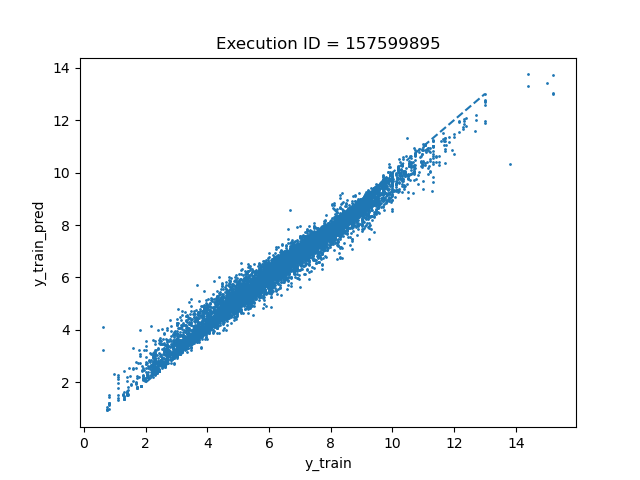
\includegraphics[scale=0.7]{accuracy_train}

\section{Machine Learning Models}
\label{MachineLearningModelslabel}
We decided to use the following machine learning models for our problem:
\begin{itemize}
\item Linear Regression
\item Support Vector Regression
\item Rotation Forest Regression
\item Random Forest Regression
\end{itemize}

By far the most impressive performance was given by Random Forest Regression.
Hence we spent more time on Random Forest regression to understand the reasons for its performance.

Because of the lack of data, Deep Neural Networks were not suitable for our problem. 
For example, if we used all the features to train a simple DNN model of size $[457,  20, 10,  1]$,  there would be 9350 parameters to train.  As we only have 16,000 data points to train our model,  the deep learning model would over-fit drastically.


\subsection{Data Preprocessing}
Before fitting the model, we did a preliminary analysis of our data.  This was necessary to train our models more reliably.

\subsubsection{Data cleaning}
Using Principle component analysis (PCA) each feature's contribution in the variation of the data was analysed. 
During this analysis 2 issues were found:
\begin{itemize}
\item There was a ligand feature named IPC that was having extremely small and extremely huge values e.g $k * 10^{39}$ where $k \in (0,1]$ .
Hence we scaled this feature using a logarithm function.
This was done for the numerical safety during the training of our models.
The affect of this scaling on the cumulative PCA is shown in Figure~\ref{fig:PCAAnalysis}. 

\begin{figure}
     \centering
     \begin{subfigure}[b]{0.45\textwidth}
         \centering
    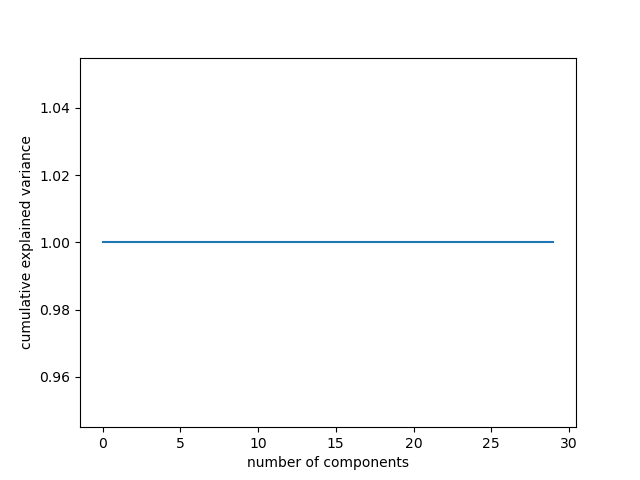
\includegraphics[scale=0.5]{images/pcaligandanalysisIPC}
    \caption{With original Ligand feature IPC}
    \label{fig:pcaproteinanalysisIPC}
     \end{subfigure}
     \hfill
     \begin{subfigure}[b]{0.45\textwidth}
         \centering
        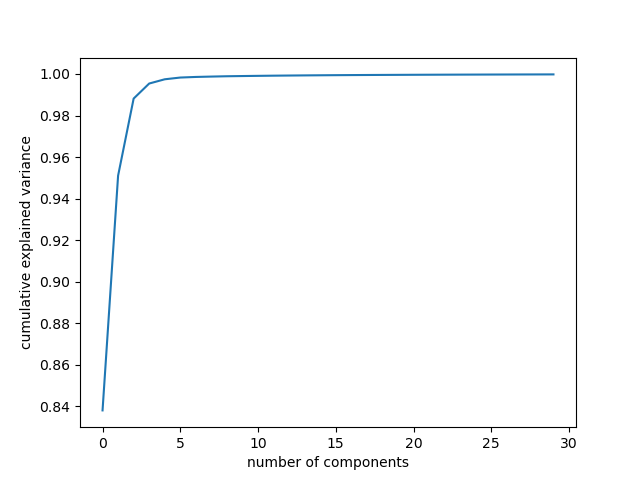
\includegraphics[scale=0.5]{images/pcawithscaledIPC}
        \caption{With log scaled Ligand feature IPC}
        \label{fig:pcawithscaledIPC}
     \end{subfigure}
     \caption{Cumulative PCA of ligand features}
     \label{fig:PCAAnalysis}
\end{figure}

\item There were a lot of NaN (Not a number) and zeros in our data.  Perhaps this was because the measurements done in the experiments were not recorded completely and the RDKit feature extracter could not extract these values relaibly. While the presence of 0s was harmless,  we made sure that we removed all NaN values before we input the data to our model.  Figure~\ref{fig:pcaproteinanalysis} shows cumulative PCA of the protein features. 
\end{itemize}

\begin{figure}[htb]
  \centering
    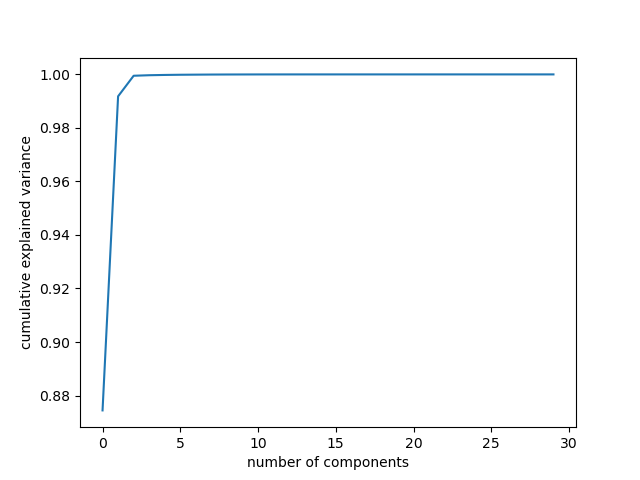
\includegraphics[scale=0.7]{images/pcaproteinanalysis}
    \caption{cumulative PCA of protein features}
    \label{fig:pcaproteinanalysis}
\end{figure}

It must be noted that,  the scaling of ligand feature IPC must be done before we use the model for prediction of new data.
This is a limitation of our model.

\subsubsection{Dealing with measurement resolution}
During the measurement of the Protein-Ligand complexes,  the measurements can be taken at various resolutions (in \si{\angstrom} units).
The accuracy of the measurement is inversely proportional to the resolution.
As shown in a small excerpt of the PDB Databank INDEX file,  we have a resolution measurement for each of the complexes (or datapoints).

\begin{verbatim}
# ==============================================================================
# List of protein-ligand complexes with known binding data in PDBbind v.2019
# 17679 protein-ligand complexes in total, sorted by binding data
# Latest update: Dec 2019
# PDB code, resolution, release year, -logKd/Ki, Kd/Ki, reference, ligand name
# ==============================================================================
3zzf  2.20  2012   0.40  Ki=400mM      // 3zzf.pdf (NLG)
3gww  2.46  2009   0.45  IC50=355mM    // 3gwu.pdf (SFX)
1w8l  1.80  2004   0.49  Ki=320mM      // 1w8l.pdf (1P3)
\end{verbatim}

Using the resolution, we devised the following 2 ways to calculate the weight of each data point.
\begin{itemize}
\item Hyperbolic formula: $  W_i = \frac{ \mathrm{\max{R_{1 ...  n}}}}{R_i}  $
\item Linear formula: $ W_i = (\mathrm{\max{R_{1 ...  n}}} + 1) - R_i $
\end{itemize}

Where $R_i$ is a resolution of a given data point.
We found that $\mathrm{\max{R_{1 ...  n}}} \approx 5$ \si{\angstrom} in our data.
It is necessary to add 1 to the max resolution in the linear formula to avoid data points with 0 weight.
The formulae are depicted in the Figure~\ref{fig:graphingformula}.
Figure~\ref{fig:resolutiondistribution} shows the distribution of data points as a function of resolution.
The resolution of the measurements ranges from 1 to 5 approximately.

\begin{figure}
     \centering
     \begin{subfigure}[b]{0.45\textwidth}
         \centering
    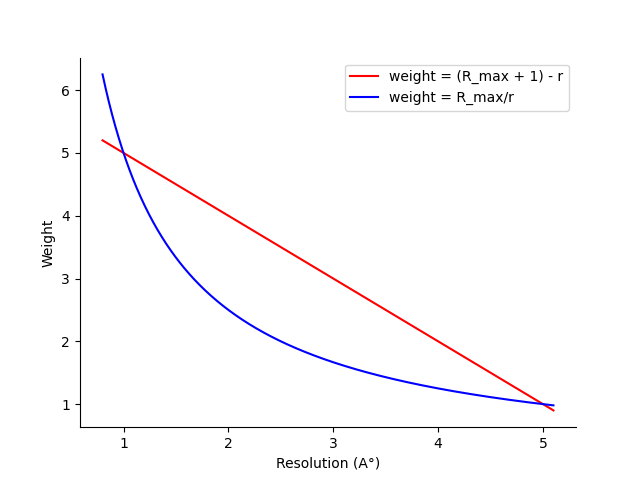
\includegraphics[scale=0.5]{images/graphingformula}
    \caption{Weight calculation formulae}
    \label{fig:graphingformula}
     \end{subfigure}
     \hfill
     \begin{subfigure}[b]{0.45\textwidth}
         \centering
        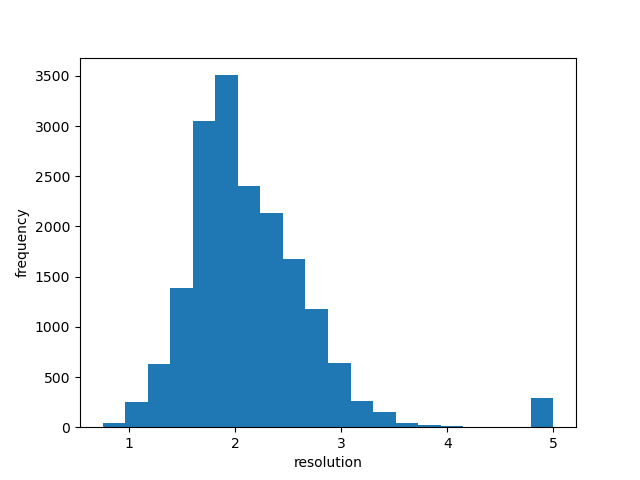
\includegraphics[scale=0.5]{images/resolutiondistribution}
        \caption{Resolution distribution}
        \label{fig:resolutiondistribution}
     \end{subfigure}
     \caption{ Weight calculation and resolution distribution}
     \label{fig:ResolutionWeightStats}
\end{figure}

Figure~\ref{fig:WeightDistribution} shows the distribution of the weights obtained from our data for linear and hyperbolic case.
In Figure~\ref{fig:linearweightdistribution},  we see that linear weighting gives us datapoints with a higher weight as compared to hyperbolic weighting.
This makes intuitive sense because as shown Figure~\ref{fig:resolutiondistribution}, 
most of the data points have a resolution around 2 \si{\angstrom}.
Since linear weighting around 2 \si{\angstrom} is higher, the linearly weighted data points will have a higher weight on average.

\begin{figure}
     \centering
     \begin{subfigure}[b]{0.45\textwidth}
         \centering
    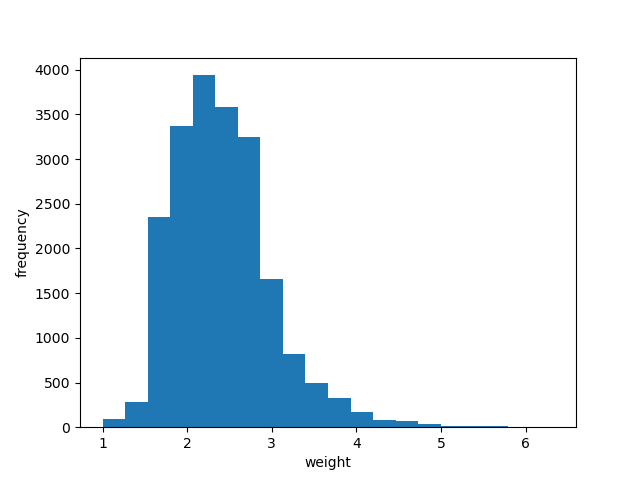
\includegraphics[scale=0.5]{images/hyperbolicweightdistribution}
    \caption{Hyperbolic weighting}
    \label{fig:hyperbolicweightdistribution}
     \end{subfigure}
     \hfill
     \begin{subfigure}[b]{0.45\textwidth}
         \centering
        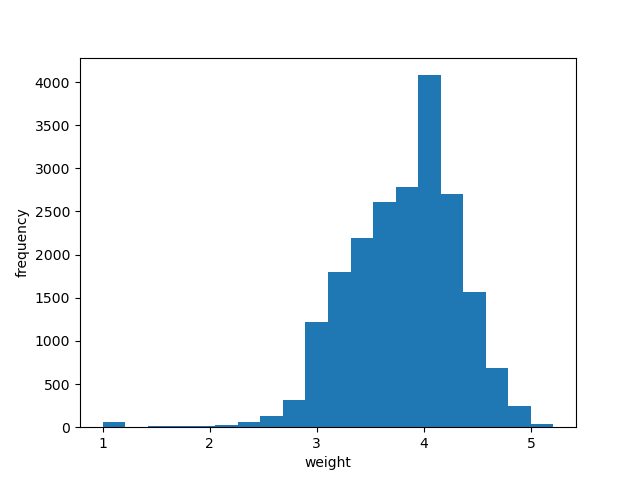
\includegraphics[scale=0.5]{images/linearweightdistribution}
        \caption{Linear weighting}
        \label{fig:linearweightdistribution}
     \end{subfigure}
     \caption{Weighting of our data points (Excluding the test set)}
     \label{fig:WeightDistribution}
\end{figure}

We employed 2 strategies to use the calculated weights in our models.

\begin{itemize}
\item Duplicating the data points.
\item Using the weights directly in the fit function.
\end{itemize}

After the duplication, we get $\approx$39,000 data points for the linear weighting formula and training and  $\approx$62,000 for the hyperbolic weighting.

\subsection{Linear regression}
Linear regression fits a linear model to a given data.
It tries to minimize the square of errors between the predicted output value and the actual output value.
This is the cheapest model (computationally) that we used to fit our data.
Table~\ref{table:1} shows the overview of our analysis with this model.
Figure~\ref{fig:BestLinearModel} shows the best results obtained with linear regression.

\begin{table} [h!]
\centering
 \begin{tabular}{ | c | c | c | c | }
\hline
\textbf{Features Selected} & \textbf{Training $R^2$ Score} & \textbf{Validation $R^2$ Score} \\ [0.5 ex]
\hline \hline
457 (all) & 0.458 & 0.414\\
457 (Hyperbolic weighting) & 0.454 & 0.428\\
457 (Linear weighting) & 0.456 & 0.430 \\
50 (Genetic - Random init)\footnotemark[1] & $\approx$0.379 & $\approx$0.359\\
49 (Genetic - Specific init)\footnotemark[1] & $\approx$0.378 & $\approx$0.368  \\
- (Output Correlation)\footnotemark[1] & - & -  \\ 
176 (manual) & 0.365  & 0.342  \\ [1ex]
\hline
\end{tabular}
\caption{Simple linear model overview}
\label {table:1}
\end{table}

\begin{figure}
     \centering
     \begin{subfigure}[b]{0.45\textwidth}
         \centering
         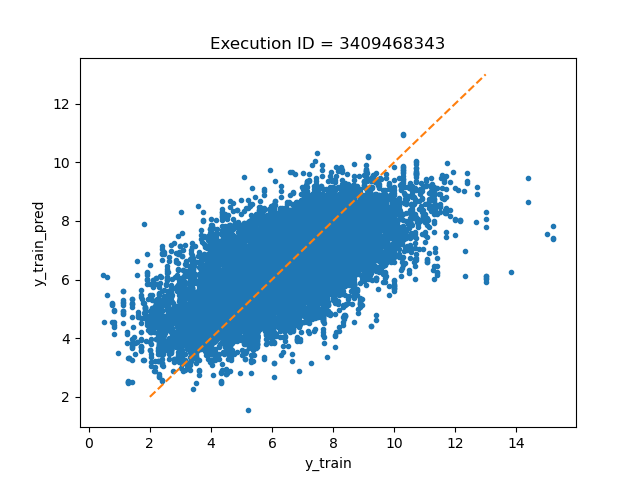
\includegraphics[scale=0.45]{images/accuracy_train_all_linear}
         \caption{Training Accuracy ($R^2 \approx 0.458$)}
        \label{fig:TrainingAccuracyLinearModel}
     \end{subfigure}
     \hfill
     \begin{subfigure}[b]{0.45\textwidth}
         \centering
         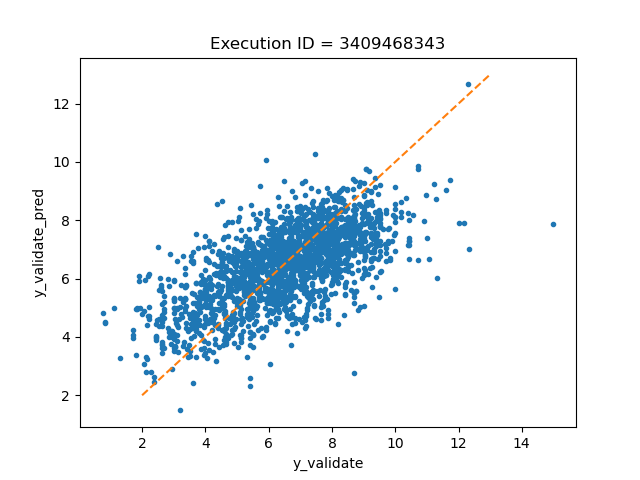
\includegraphics[scale=0.45]{images/accuracy_validate_all_linear}
        \caption{Validation Accuracy ($R^2 \approx 0.414$)}
        \label{fig:ValidationAccuracyLinearModel}
     \end{subfigure}
     \caption{Best Linear Model.  All 457 features selected.}
     \label{fig:BestLinearModel}
\end{figure}

The reason for the low $R^2$ score is that linear models assume a strong linearity between the input variables and the output variable.
This is not always true.

In the linear regression model,  we used genetic algorithms to reduce both the large feature space and to eliminate correlated features within the families. 

\subsubsection{Score function of genetic feature selection}
\label{GenerationScoringFunction}
Since the fitting of the linear regression model was very cheap, we could afford to refit the model every time in our genetic algorithm.
We had 2 objectives at hand
\begin{itemize}
\item Get the best performing model.
\item Reduce the number of input features to make our model simple and explainable.
\end{itemize}
The above objectives are not always against each other.
This is because removing a feature that has no correlation (or random correlation) with the output may improve the model whereas removing a feature that the output is highly correlated on degrades the model.

\footnotetext[1]{Approximately reproducible as the reproducibility module was introduced later.}

Hence,  taking inspiration from the hypervolume-based multi-objective optimization, we designed the following score function.
$$
\textrm{score} = \mathbf{R}^2 \textrm{score} * \textrm{Features Eliminated}
$$
Figure~\ref{fig:scorefunctionfigure} gives us an intuition about this function.
Here the score function represents the area of the square formed between a given point and the origin.
Trying to improve the score means,  it will try to eliminate more features as well as try to get a higher $R^2$ score.
In the example below,  the point $a$ is preferred over $b$ as it gives almost the same $R^2$ score and eliminates a larger number of features.
Another advantage of this score function is that the scale of both axes is irrelevant.

\begin{figure}[htb]
  \centering
    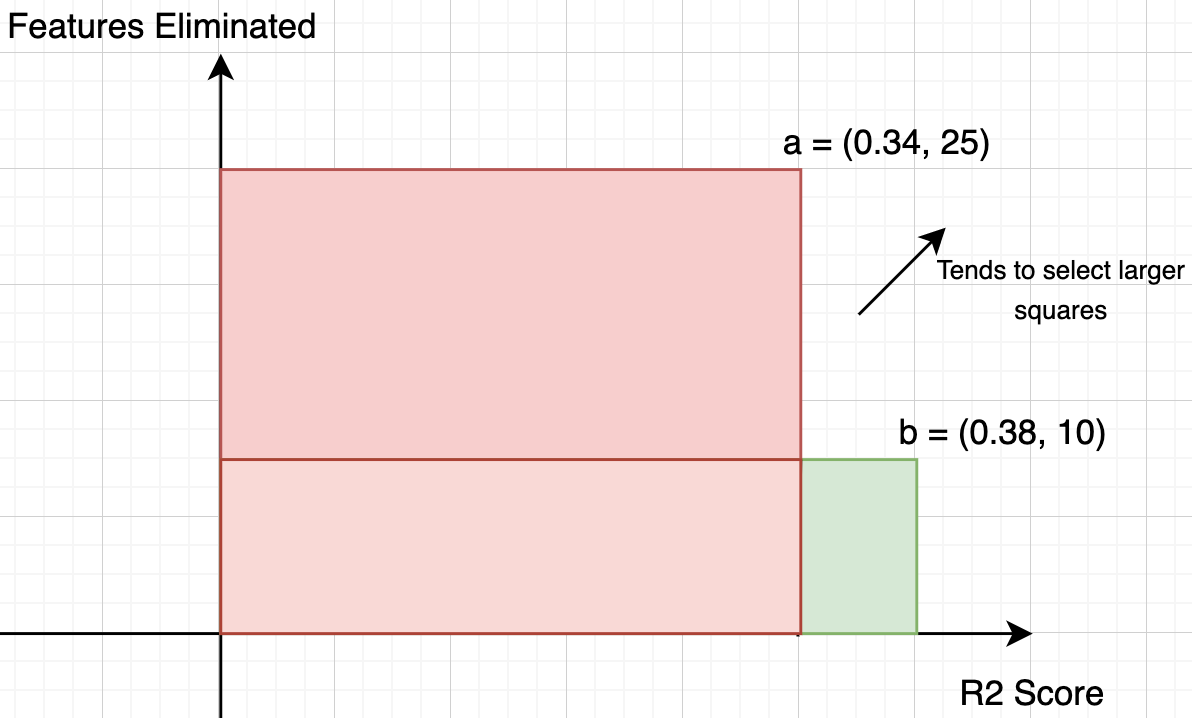
\includegraphics[scale=0.5]{images/scoreFuntionMultiObject}
    \caption{Genetic Algorithm score function representation.}
    \label{fig:scorefunctionfigure}
\end{figure}

\subsubsection{Initialization strategies of population}
Two main strategies were used to initialize the population for the genetic algorithm
\begin{itemize}
\item \textbf{Random Initialization}.  A population of $2400$ chromosomes was randomly initialized and run for $500$ generations.
\item \textbf{Specific Initialization}.  Here,  the initial population was kept at $457$.
The algorithm was run for $2000$ generations.
Each chromosome in the population had 1 distinct feature excluded.  The following represents the initialization of the chromosomes.

$
c_1 = [0 1 1 1 1 ......  1 1]
$ \\
$
c_2 = [1 0 1 1 1 ......  1 1]
$ \\
$
c_3 = [1 1 0 1 1 ......  1 1]
$ \\
$
... 
$ \\
$
c_{457} = [1 1 1 1 1 ......  1 0]
$

The rationale was that using the above score function we could go to a local minimum by eliminating the worst performing features rather than trying to select the best performing features as in the case of random initialization.
\end{itemize}

Both the initialization strategies gave similar results as shown in Table~\ref{table:1}

\subsection{Random Forest Regression}
Random forest regression is an ensemble ML model of regression trees.
When training each tree,  the algorithm finds out which feature value can divide the data into 2 groups to yield the lowest sum of squared values on both sides (The criterion can be different as well e.g. lowest absolute error).
Then each of the sub-data is split recursively till a stopping criterion (e.g a set number of data points in the leaf).

For each tree,  a subset of the data is used for training. 
The subset of data is sampled with replacement a.k.a bagging.
After training,  the bunch of "Experts" that are good at different data subsets predict the output of new given inputs.
The average of the predicted outputs is the result of the whole random forest regressor.

This model is non-linear.
One advantage is that there is no need for any assumption about the data.
Moreover,  random forests can handle categorical features together with the real-valued features very easily.
On the negative side,  the function represented by the ensemble cannot be easily represented and has to be interpreted as a black-box function.

Figure~\ref{fig:RFMModel} shows the validation and accuracy results obtained by a random forest of 100 trees when we use all the 457 features as input.
As you can see,  this model far outperforms the linear one.

The following table gives you an overview of our model.

\begin{table} [h!]
\centering
 \begin{tabular}{ | c | c | c | c | }
\hline
\textbf{Features Selected} & \textbf{Training $R^2$ Score} & \textbf{Validation $R^2$ Score} \\ [0.5 ex]
\hline \hline
457 (all) & 0.310 & 0.295\\
457 (Hyperbolic weighting) & 0.334 & 0.302\\
457 (Linear weighting) & 0.456 & 0.430 \\
- (Output Correlation)\footnotemark[1] & - & -  \\ 
- (Genetic Elitism) & 0.456 & 0.430 \\
- (Genetic Normal) & 0.456 & 0.430 \\
176 (manual) & 0.365  & 0.342  \\ [1ex]
\hline
\end{tabular}
\caption{Random Forest Regression overview}
\label {table:3}
\end{table}

\begin{figure}
     \centering
     \begin{subfigure}[b]{0.45\textwidth}
         \centering
         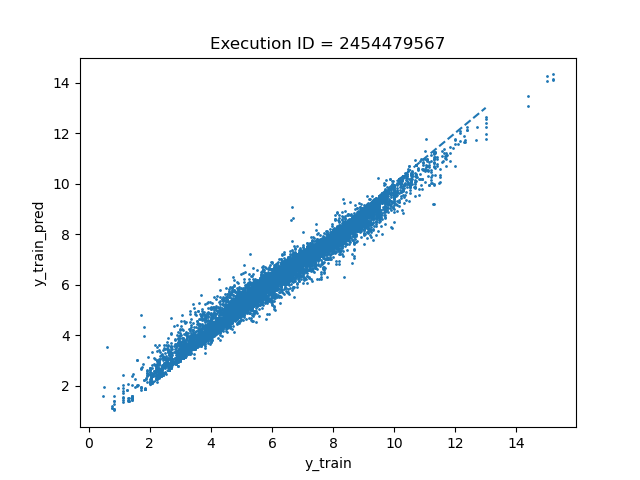
\includegraphics[scale=0.45]{images/accuracy_train_rfr}
         \caption{Training Accuracy ($R^2 \approx 0.971$)}
        \label{fig:TrainingAccuracyRFM}
     \end{subfigure}
     \hfill
     \begin{subfigure}[b]{0.45\textwidth}
         \centering
         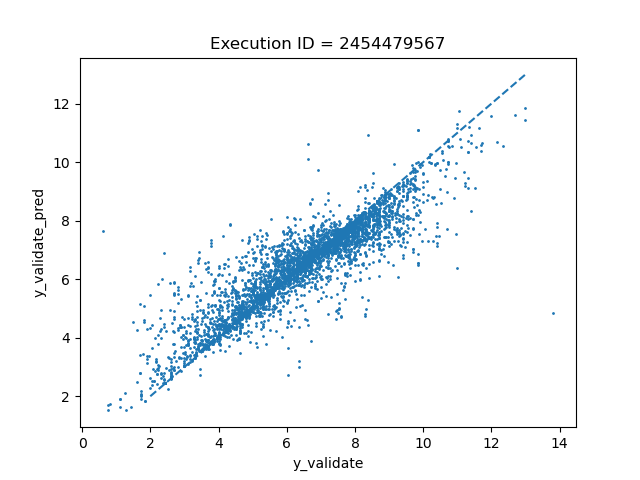
\includegraphics[scale=0.45]{images/accuracy_validate_rfr}
        \caption{Validation Accuracy ($R^2 \approx 0.797$)}
        \label{fig:ValidationAccuracyRFM}
     \end{subfigure}
     \caption{Random Forest Regressor with 457 features and 100 trees.}
     \label{fig:RFMModel}
\end{figure}

\subsubsection{Dealing with correlated features}
In Section \ref{CorrelationAnalysis} we discussed that within some the families of features there are heavily correlated features.
One way to deal with this would be to just taken one feature from a family and exclude the rest.
However this would not be a good strategy for generalization.
This is because in future,  if this one feature is not measured,  our model would be rendered useless.

For this reason,  we made use of the stochasticity of the random forest to our advantage.
During the creation of a regression tree,  the random forest model tries to get the best (feature,  value) tuple to divide the data. This is known as the split criteria.
We force it to randomly select only 20\% of the features for deciding on the split criteria.
More specifically,  we use the following values
\begin{itemize}
\item 400 Trees (n\_estimators)
\item 20\% of feature selection.  (max\_features)
\item A minimum of 2 data points for each leaf.  (min\_samples\_leaf)
\end{itemize}
These hyper-parameters were determined after some empirical testing.
We increased the number of estimators as we increased the stochasticity of our ensemble.
Our model would hence be dependent on the entire family of features and not rely on a single feature heavily.

\subsubsection{Dealing with measurement resolution}

We trained our model by duplicating the data according to their weights. 
After training we got the following results - Training $R^2$ score = 0.995,  Validation $R^2$ score = 0.8298 and  Out of bag (oob) score = 0.977.

We found the following issues with this strategy:
\begin{itemize}
\item The out of bag error (oob score) is erroneously high here. This is because of repeated data points. Many points are both inside the selected bag and outside it.
\item Due to duplication of data points,  the trees may end up being more correlated to each other.  This will affect generalization of our model.
\item As training this model is costly, duplicating the data points further increases the cost of training.
\end{itemize}
Hence, we conclude that duplication of the data based on their weights is a wrong strategy for this model.

When we used our weight directly in the fit function,  we could not get any noticable improvement in our model.
We think this is because the data is already skewed towards the $\approx$2 \si{\angstrom}
data points.
This can be seen in Figure~\ref{fig:resolutiondistribution}

\subsubsection{Feature Importance calculation}
The Random Forest regression model fitting is very expensive as compared to the simple linear regression.
Hence the same strategy cannot be used for feature selection as used in the linear models.
We used the following strategies to determine the importance of features in the model.

\begin{itemize}
\item \textbf{Gini Importance (or) Decrease in impurity}.  This is calculated by the model itself.
For every feature,  it calculates how much decrease in the split criterion the feature contributes to the entire ensemble (i.e in every node its used in all the trees).
The disadvantage is that they cannot be reliable when the features have a high cardinality.  Figure~\ref{fig:GiniImportanceLabel} illustrates this importance.
\item \textbf{Permutation Importance} - This is a model agnostic method.
It tries to calculate the reduction in the accuracy we shuffle each feature.
The more the reduction the more important the feature is.
The disadvantage is that since each feature is checked independently,  correlated input features make the results unreliable. 
If feature $A$ and feature $B$ are correlated,  the shuffling of $A$ may not impact the model as the model can rely on $B$ for its prediction.  Figure~\ref{fig:PermutationImportanceLabel} illustrates this importance.
\end{itemize}

\begin{figure}
     \centering
     \begin{subfigure}[b]{0.45\textwidth}
         \centering
         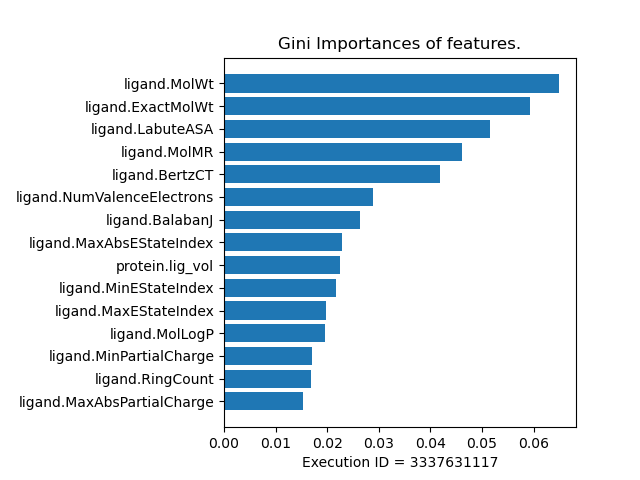
\includegraphics[scale=0.45]{images/Gini_importance}
         \caption{Gini importance}
        \label{fig:GiniImportanceLabel}
     \end{subfigure}
     \hfill
     \begin{subfigure}[b]{0.45\textwidth}
         \centering
         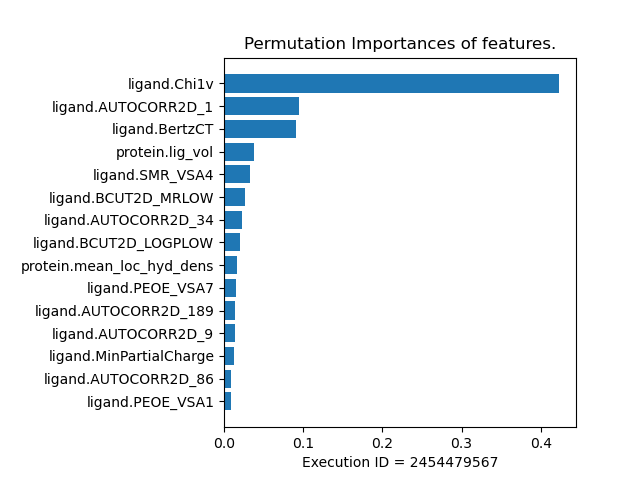
\includegraphics[scale=0.45]{images/Permutation_importance}
        \caption{Permutation importance}
        \label{fig:PermutationImportanceLabel}
     \end{subfigure}
     \caption{Feature Importance calculation of Random Forest Regressor}
     \label{fig:RFMFILable}
\end{figure}

\subsubsection{Permutation Importance and genetic algorithm}
To overcome the issue with the above feature importance selection, we plan to use a combination of the concepts of permutation importance and genetic algorithm to find out the importance of the selected features.
This is because it is very expensive to refit the model and cheap enough to check the results of shuffling the model.

We used 2 different strategies to get the for our genetic algorithms -
\begin{itemize}
\item \textbf{Using specific scoring function}.  In Section ~\ref{GenerationScoringFunction},  we discussed intuition behind the scoring function used in our genetic model.
In the random forest model,  however,  this scoring function selected a lot of features ($> 400$). Hence we researched the following scoring function in an effort to reduce the number of features. 
$$
\textrm{score} = R_2 score * \textrm{Features Eliminated}^2
$$
We used a a stronger signal for the number of eliminated features. This scoring function, however,  turned out to be too strong and non of the features were selected.
\item \textbf{Elitism}.  Elitism is a strategy used in the genetic algorithms to select the top few elements from each generation for the next generation in addition to the newly created children. This keeps the best performing subset of the population always in the current generation in an effort to improve them further by cross over or mutation.
\end{itemize}


\subsection{Support Vector Regression}
Support vector regression is a non-linear regression method that fits a curve such that the margin of error between the model's prediction and the original value is kept within a minimum range.
Any error higher than this minimum range is penalised during training of the model.
We trained support vector regression with the RBF kernel.

\begin{table} [h!]
\centering
 \begin{tabular}{ | c | c | c | c | }
\hline
\textbf{Features Selected} & \textbf{Training} & \textbf{Validation} &  \textbf{Testing} \\ [0.5 ex]
\hline \hline
457 (all) & 0.314 & 0.279 & 0.318\\
457 (Hyperbolic weighting) & 0.333 & 0.304 & 0.341\\
\textbf{457 (Linear weighting)} & \textbf{0.342} &\textbf{0.323} & \textbf{0.349}\\
- (Output Correlation)\footnotemark[1] & - & -  & - \\ 
176 (manual + Linear weighting) & 0.308  & 0.286  & 0.314\\ [1ex]
\hline
\end{tabular}
\caption{Table showing  $R^2$ Scores for SVR}
\label {table:2}
\end{table}

We did not use the duplication of data strategy for this model because the training time complexity is $O(n^2)$ where n is the number of data points.
However,  we did use data point weights during the fit function of the training.

The results are reported in Table~\ref{table:2}.
The linear weighting of the data gave the best results in SVR.
The reason testing $R^2$ score is around the same range as the training score may be because the testing data is of better better quality data as compared to the validation data.
However this can vary slightly based on the random seed used.

As the performance of the model was not on par with other models,
we did not run the costly genetic algorithm feature selection on SVR.
Moreover,  the time it took to get the $R^2$ score (validation and testing) was very high and was not suitable to be used in permutation based genetic algorithm as discussed in the random forest section.
The issues of within family feature correlation as well as feature selection were hence dealt by either using output correlation or by manual feature selection.

Figures~\ref{fig:accuracyvalidateSVRLinear} and ~\ref{fig:accuracytestSVRLinear} visualize the training and validation error of the best model.

\begin{figure}
     \centering
     \begin{subfigure}[b]{0.45\textwidth}
         \centering
         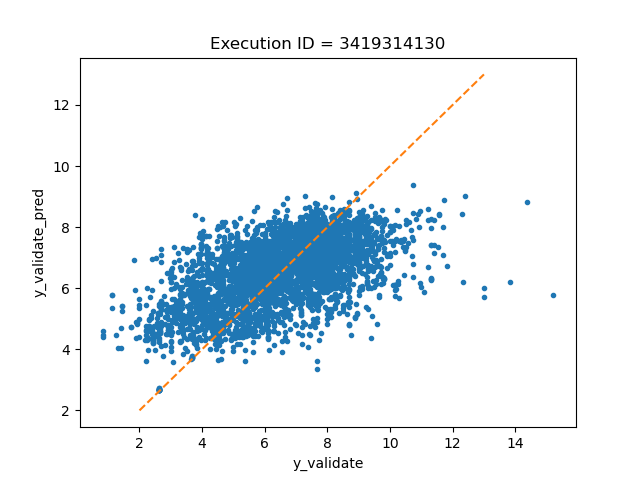
\includegraphics[scale=0.45]{images/accuracyvalidateSVRLinear}
         \caption{accuracyvalidateSVRLinear}
        \label{fig:accuracyvalidateSVRLinear}
     \end{subfigure}
     \hfill
     \begin{subfigure}[b]{0.45\textwidth}
         \centering
         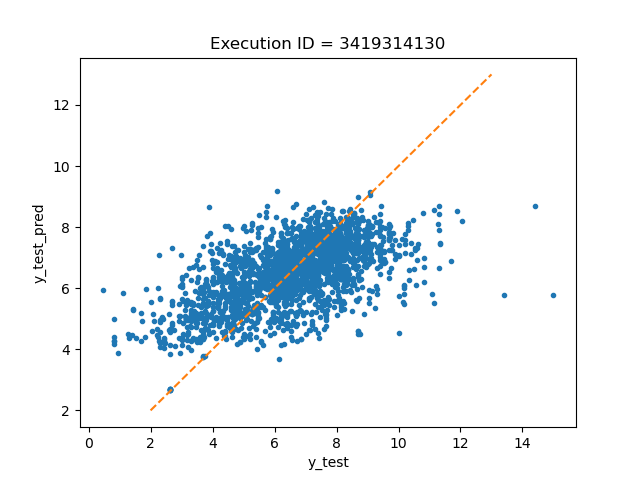
\includegraphics[scale=0.45]{images/accuracytestSVRLinear}
        \caption{accuracytestSVRLinear}
        \label{fig:accuracytestSVRLinear}
     \end{subfigure}
     \caption{SVR accuracy visualization for 457 (Linear weighting) feature selection}
     \label{fig:SVRaccuracy}
\end{figure}


\subsection{Rotation Forests}

The training $R^2$ score was comparable to that of random forest regressor.
However, this did not yield good validation error.
One of the reasons,  we hypothesize,  is that rotation forest are shown to be better than random forest only for the continuous feature values.
However,  as per the domain expert,  we may have many discrete values in our feature space.
Hence we conclude that this model is not the best model for our problem.

\begin{table} [h!]
\centering
 \begin{tabular}{ | c | c | c | c | }
\hline
\textbf{Features Selected} & \textbf{Training $R^2$ Score} & \textbf{Validation $R^2$ Score} \\ [0.5 ex]
\hline \hline
457 (all) & 0.310 & 0.295\\
457 (Hyperbolic weighting) & 0.334 & 0.302\\
457 (Linear weighting) & 0.456 & 0.430 \\
- (Output Correlation)\footnotemark[1] & - & -  \\ 
- (Genetic Elitism) & 0.456 & 0.430 \\
- (Genetic Normal) & 0.456 & 0.430 \\
176 (manual) & 0.365  & 0.342  \\ [1ex]
\hline
\end{tabular}
\caption{Rotation Forest overview}
\label {table:4}
\end{table}

\section{Discussion}
In this project,  we tried to determine the protein-ligand binding affinity by using spacial features extracted by RDKit and dpocket.
We believe that the presence of 2D/3D features made our data more accesible to simple machine learning models. 
This was crucial because the complex models that directly get the 3D features from the data (e.g. 3D convolutions) require huge amount of data which is expensive to accumulate.

We spent most of the time analysing and studying the most suitable linear model (Linear Regression) and non-linear model (Random Forest Regression) for our extracted data.
Our study also included feature selection methods like genetic algorithms.
We found that our extracted protein ligand data had the following interesting properties
\begin{itemize}
\item The data does not not have a symmetric Gaussian distribution.  In other words, the ranges of values in each dimension were very different.
\item The features are both real valued numbers as well as discrete.  The discrete values are also represented as real numbers.
\item There are feature families in the ligand descriptors that have features that are highly correlated.
\end{itemize}

While linear regression did give reasonable results,  it was not a very reliable model because it assumed that the data was linearly related to the binding affinity.
Nevertheless,  we were able to run genetic algorithms on this model to get the best $\approx$ 50 features.
We failed to do this in case of the Random Forest Regression model.

From our study of genetic genetic algorithms we make the conclusion that it was not very helpful in improving the performance of our model. However we were able to reduce or eliminate around 50 features for the Random Regression Model and around 400 features in the linear Regression without hampering the performance to a large degree.
One issue we found with genetic algorithms is that they make the model very reliant on the selected features.
This hard constraint may not be good when data collection process is expensive and error prone.

We found that the Random Forest Regression was able to deal with all the above specific properties of our data.
Random Forest Regression deals with both Real valued and discrete input features because the main aim of a fitting tree (in the random forest) is to reduce the entropy of the divided data.
Since all the discrete features in our data are represented as real valued number,  the trees can can easily find a midpoint between the discrete values to divide the data. 
Interestingly,  we could also use the feature correlation within families to our advantage to improve the robustness of our model. 
By increasing the randomness of our feature selection during the data split we force our model to rely less on a specific feature.
Hence a wrong measurement or a corrupted feature would not hamper our model significantly.

Since we are getting an $R^2$ score of $>$ 0.65 consistently,  the binding affinity predicted by our model can be used for any new PL complex can be taken as a reference for drug-testing decisions.
For example,  one can use the results to prioritize testing of new ligands in a wet lab experiment to save resources for the important ligands.

As with any model,  our model and approach does have limitations. 
Firstly our model cannot be explained very easily.
With hundreds of trees in our random forest, the model can only be treated as a Black Box.
Because of the complexity of our model,  we were not able to show why some features were very important and other not so important - for example in the feature importance calculation.
Secondly, our model relies heavily on the ligand features. 
This makes our model assume that the binding only slightly depends on the protein which is not the case conceptually.
Also, we could not perform hyper-parameter optimization,
in conjunction with the genetic feature selection algorithms as it is prohibitively expensive.

\section{Conclusion}
In this project we studied methods and preprocessing techniques to predict the protein ligand binding affinity.
In conclusion we would like to suggest the use of Random Forest Regression for this problem because of the ease training and its generalization capability.
We believe that a random forest regression,  could be used as a baseline to compare any new models.

In further work,  we believe that there is scope for improving the feature selection process of our model.
One issue which could not be solved by us is that our model uses more ligand features than protein features.
Further study on why this is the case would be helpful.
One way could be to build models with all protein features and one family of ligand features. 
The most important features in each family may be used as surrogates for the whole family.
We also think more study needs to be conducted to create explainable models.
This would be both accepted by the cheminformatics community and would be helpful to further the understanding of binding affinity.

\bibliographystyle{plain}
\bibliography{references}

\section{Appendix}
\subsection{XYZ File format}
\label{XYZFileexampleref}
The following represents the pyridine molecule in the XYZ format.
\begin{verbatim}
11

C       -0.180226841      0.360945118     -1.120304970
C       -0.180226841      1.559292118     -0.407860970
C       -0.180226841      1.503191118      0.986935030
N       -0.180226841      0.360945118      1.29018350
C       -0.180226841     -0.781300882      0.986935030
C       -0.180226841     -0.837401882     -0.407860970
H       -0.180226841      0.360945118     -2.206546970
H       -0.180226841      2.517950118     -0.917077970
H       -0.180226841      2.421289118      1.572099030
H       -0.180226841     -1.699398882      1.572099030
H       -0.180226841     -1.796059882     -0.917077970
\end{verbatim}

\subsection{SDF File format}
\label{SDFFileexampleref}
\begin{verbatim}
2uzn_ligand

Created by X-TOOL on Fri Nov 18 14:55:27 2016
 37 39  0  0  0  0  0  0  0  0999 V2000
    7.1480   60.4530    6.6830  O 0  0  0  1  0  1
    6.0470   60.1670    7.5640  S 0  0  0  1  0  4
    .......
    .......
   -2.6338   67.4589    8.1225  H 0  0  0  1  0  1
  1  2  2  0  0  2
  2  3  2  0  0  2
  .......
  .......
 23 37  1  0  0  2
M  END
> <MOLECULAR_FORMULA>
C15H13N3O4S2

> <MOLECULAR_WEIGHT>
363.3

> <NUM_HB_ATOMS>
7  

> <NUM_ROTOR>
1  

> <XLOGP2>
1.31 
\end{verbatim}

\subsection{MOL2 File Format}
\label{MOL2Fileexampleref}
\begin{verbatim}
### 
### Created by X-TOOL on Fri Sep 26 17:34:18 2014
### 

@<TRIPOS>MOLECULE
1fo2_ligand
   25    25     1     0     0
SMALL
GAST_HUCK


@<TRIPOS>ATOM
      1 C4         39.0090   40.2680   25.5130 C.3       1 DMJ         0.1280
      2 O4         39.2170   40.5810   26.8980 O.3       1 DMJ        -0.3835
     .......
     25 H14        38.0787   41.8134   21.3802 H         1 DMJ         0.2097
@<TRIPOS>BOND
     1    1    9 1  
     2    1    3 1  
    .......
    25   11   25 1  
@<TRIPOS>SUBSTRUCTURE
     1 DMJ         1
\end{verbatim}

\subsection{Correlation Heat Maps}
\label{CorrHeatMapsAppendix}
This section shows the correlation heat maps of the most interesting feature families in the our dataset.
\begin{figure}
     \centering
     \begin{subfigure}[b]{0.45\textwidth}
         \centering
    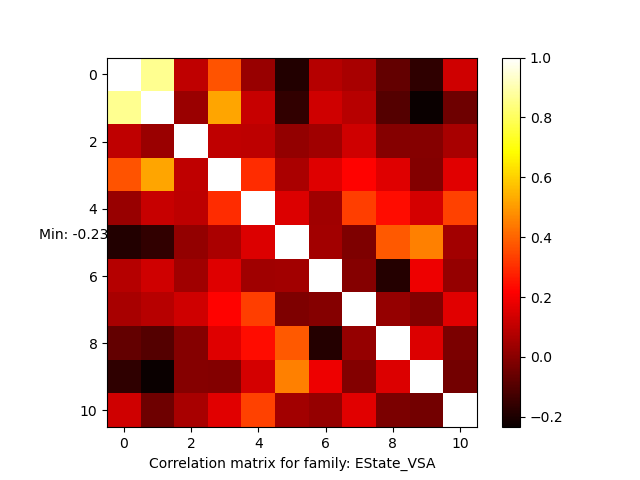
\includegraphics[scale=0.5]{images/correlationEStateVSA}
    \caption{Family EState\_VSA}
    \label{fig:correlationEStateVSA}
     \end{subfigure}
     \hfill
     \begin{subfigure}[b]{0.45\textwidth}
         \centering
        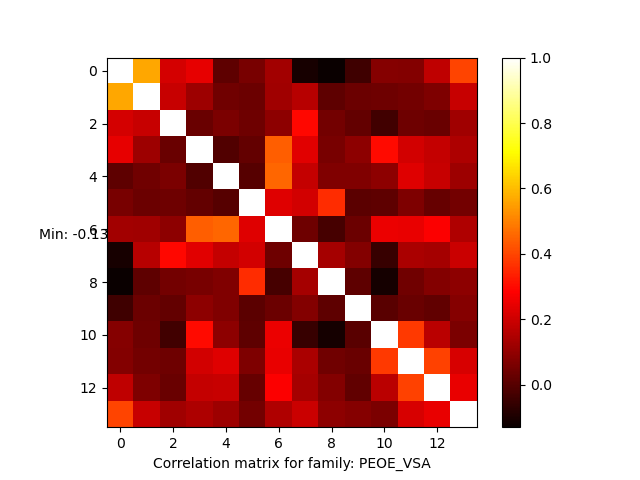
\includegraphics[scale=0.5]{images/correlationPEOEVSA}
        \caption{Family PEOE\_VSA}
        \label{fig:correlationPEOEVSA}
     \end{subfigure}
          \hfill
     \begin{subfigure}[b]{0.45\textwidth}
         \centering
        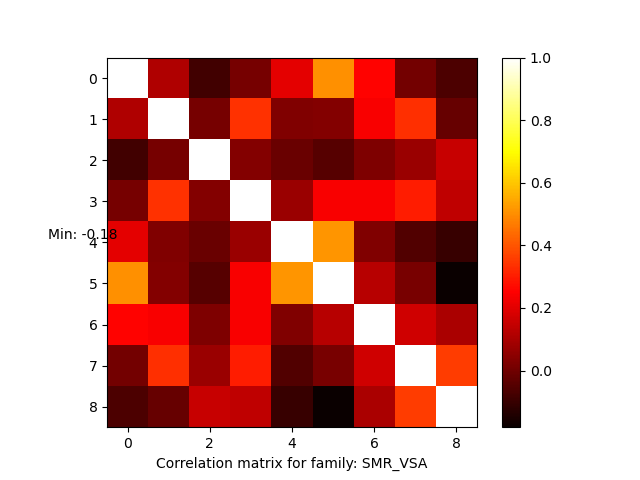
\includegraphics[scale=0.5]{images/correlationSMRVSA}
        \caption{Family SMR\_VSA}
        \label{fig:correlationSMRVSA}
     \end{subfigure}
               \hfill
     \begin{subfigure}[b]{0.45\textwidth}
         \centering
        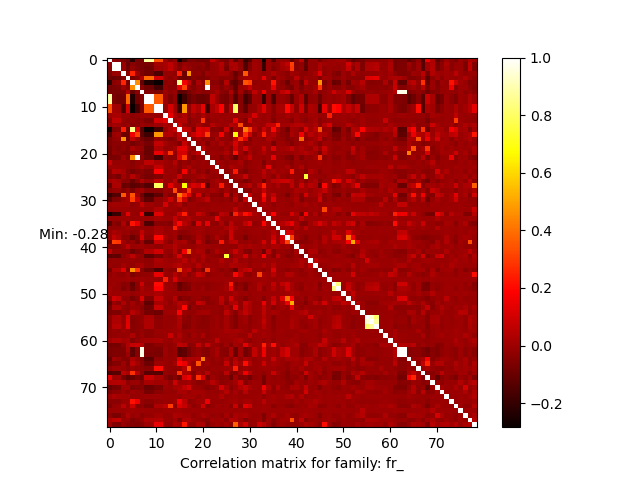
\includegraphics[scale=0.5]{images/correlationfr}
        \caption{Family fr\_}
        \label{fig:correlationfr}
     \end{subfigure}
      \hfill
     \begin{subfigure}[b]{0.45\textwidth}
         \centering
        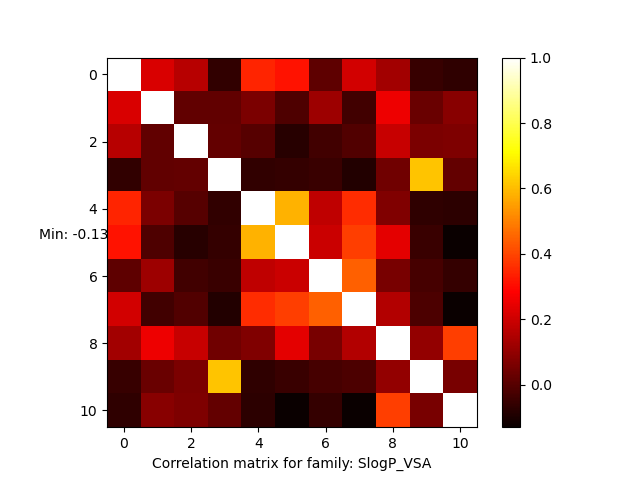
\includegraphics[scale=0.5]{images/correlationSlogPVSA}
        \caption{Family SlogP\_VSA}
        \label{fig:correlationSlogPVSA}
     \end{subfigure}
             \hfill
     \begin{subfigure}[b]{0.45\textwidth}
         \centering
        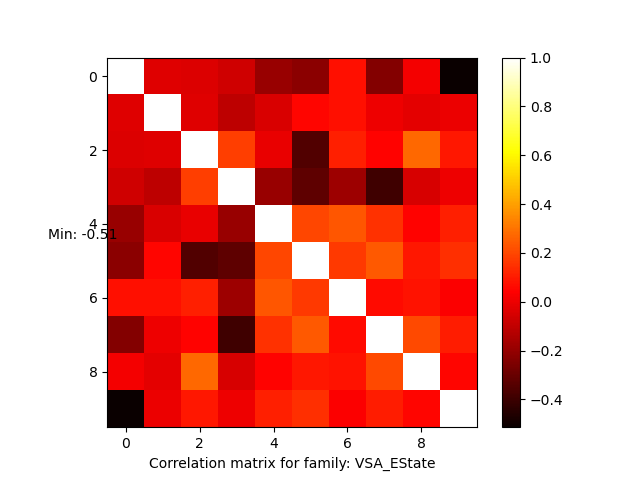
\includegraphics[scale=0.5]{images/correlationVSAEState}
        \caption{Family VSA\_EState}
        \label{fig:correlationVSAEState}
     \end{subfigure}     
     \caption{Correlation Heat Maps}
     \label{fig:CorrHeatMapFig}
\end{figure}

\end{document}
